\pgfmathsetmacro{\ra}{20}


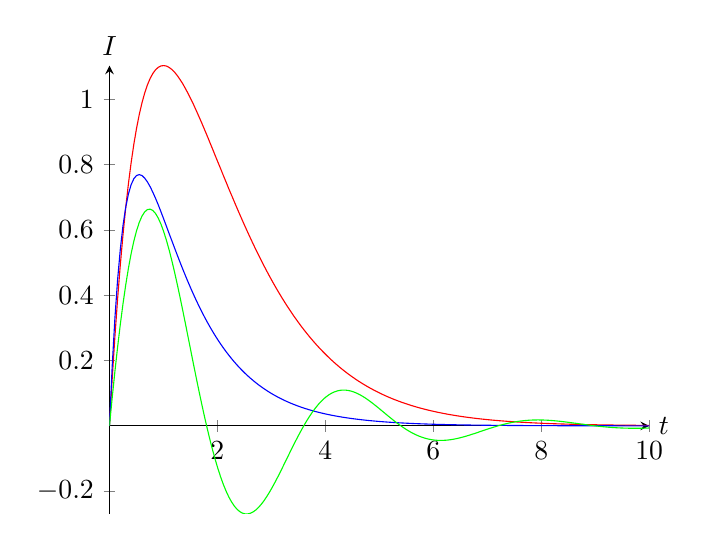
\begin{tikzpicture}
  \begin{axis}[
      axis lines=middle,
      xlabel = \(t\), xlabel style={at=(current axis.right of origin), anchor=west},
      ylabel = \(I\), ylabel style={at=(current axis.above origin), anchor=south}
      ]
    \addplot[domain=0:10, samples=200, color=red]{3 * x * exp(-x)};
    \addplot[domain=0:10, samples=200, color=blue]{2 * exp(-2 * x) * (exp(x) - exp(-x)};
    \addplot[domain=0:10, samples=200, color=green]{exp(-0.5 * x) * sin(100 * x)};


  \end{axis}
\end{tikzpicture}
